%% 30min talk

\documentclass[english]{beamer}
\usetheme{Warsaw}
\setbeamertemplate{navigation symbols}{} % remove the navigation symbols
\setbeamertemplate{headline}{} % remove headline
\setbeamertemplate{footline}[frame number]

\usepackage{babel}
\usepackage[utf8]{inputenc}
\usepackage{textcomp}
\usepackage{wasysym}

\title{Beyond-the-standard-model contributions to rare B decays analyzed with variational-Bayes enhanced adaptive importance sampling}
\author{Stephan Jahn}
\date{\today} %TODO: insert date

% ----------------------------------------------------------------------

\begin{document}

\newcommand{\slide}[2][t]{\begin{frame}[#1] \frametitle{\insertsection} #2 \end{frame}}
\newcommand{\KLPq}[0]{KL( P\|{}q)}
\newcommand{\varmuN}{var(\mu^{N})}

% ----------------------- title page, unnumbered -----------------------

{
\setbeamertemplate{footline}{}
\frame[nopagenumbering]{\titlepage}
}

% -------------------------- overview section --------------------------

\section{Overview}

\slide[t]{

    Bayes' formula:
    \newline \newline
    $$ P(\theta | \mathcal{D}, \mathrm{M} ) = \frac{P(\mathcal{D}|\theta, \mathrm{M})P(\theta | \mathrm{M})}{P(\mathcal{D} | \mathrm{M} )}
       = \frac{P(\mathcal{D}|\theta, \mathrm{M})P(\theta | \mathrm{M})}{\int P(\mathcal{D}|\theta, \mathrm{M})P(\theta | \mathrm{M}) d\theta }$$

    \only<2->{ \
        \newline \newline \
        our application: \
        \
        \newline \newline \

        \only<3->{$$ \theta = \lbrace \mathcal{C}_{7 , 9 , 10 , S , P , T , T5 , ...}^{(\prime)} \rbrace $$}
        \only<4->{$$ \mathcal{D} = \mathrm{experimental~data} $$}
        \only<5->{$$ \mathrm{M} = \mathrm{EFT , SM , ...} $$}
    }

}


\slide[t]{

{\large\textbf{Goals}}

\begin{columns}[t] % The "c" option specifies centered vertical alignment while the "t" option is used for top vertical alignment

\column{.45\textwidth} % Left column and width

\only<2->{\begin{itemize}
              \item draw marginal plots of the posterior
              \
              \newline

              \hspace{-1.2cm} 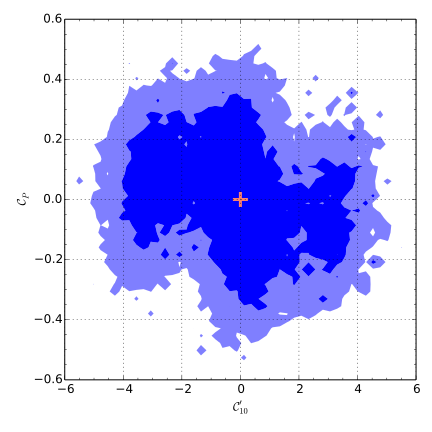
\includegraphics[width=1.01\textwidth]{figures/C10p_CP}

          \end{itemize}}

\column{.5\textwidth} % Right column and width

\only<3->{\begin{itemize}
          \item compare models $\mathrm{EFT} \leftrightarrow \mathrm{SM}$
          \end{itemize}

              $$ \frac{P(\mathrm{EFT}|\mathcal{D})}{P(\mathrm{SM}|\mathcal{D})} =
                 \frac{P(\mathcal{D}|\mathrm{EFT})}{P(\mathcal{D}|\mathrm{SM})} \cdot \frac{P(\mathrm{EFT})}{P(\mathrm{SM})} $$

              $$ P(\mathrm{M} | \mathcal{D} ) = \frac{P(\mathcal{D} | \mathrm{M})P(\mathrm{M})}{P(\mathcal{D})} $$

          \begin{itemize}
          \item[]
              \begin{itemize}
                  \item[] \only<4->{\hspace{-0.1\textwidth} $\frac{P(\mathrm{EFT}|\mathcal{D})}{P(\mathrm{SM}|\mathcal{D})} > 1$ new physics \smiley{} \newline}
                  \item[] \only<5->{\hspace{-0.1\textwidth} $\frac{P(\mathrm{EFT}|\mathcal{D})}{P(\mathrm{SM}|\mathcal{D})} < 1$ confirm SM \frownie{}}
              \end{itemize}
          \end{itemize}}

\end{columns}

}





\slide[t]{

{\large\textbf{Difficulties}}

\begin{columns}[t] % The "c" option specifies centered vertical alignment while the "t" option is used for top vertical alignment

\column{.45\textwidth} % Left column and width

\vspace{0.65cm} % to center the text

\only<2->{\begin{itemize}}
\only<2->{\item curse of dimensionality}
\only<3->{\item multimodality}
\only<4->{\item degeneracies}
\only<2->{\end{itemize}}

\only<5->{\Huge \textcolor{red}{no standard algorithm so far}}

\column{.5\textwidth} % Right column and width

\vspace{-8mm}

\begin{center}
\only<3->{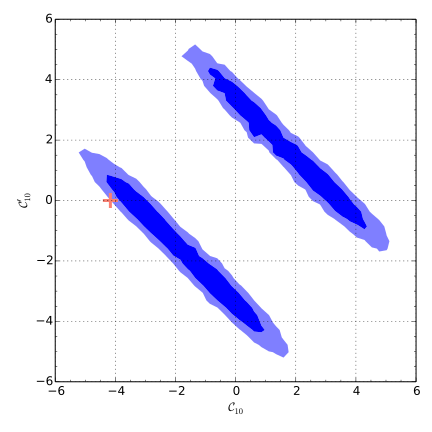
\includegraphics[height=0.4\textheight]{figures/C10_C10p}}

\only<4->{\includegraphics[height=0.43\textheight]{figures/example_for_degeneracy}}
\end{center}


\end{columns}

}

% ------------------------------ toc page ------------------------------

\begin{frame}
\frametitle{Contents}
\tableofcontents
\end{frame}

% ----------------------------- VB section -----------------------------

\section{Adaptive importance sampling with the variational-Bayes approach} %TODO: write

\slide{ %TODO: maybe short summary here; importance sampling and variational Bayes then summary at the end

    \textlangle empty\textrangle

}

\subsection{Adaptive importance sampling}

\slide{

    \frametitle{\insertsubsectionhead}

    $$ \int P(x) dx = \int \frac{P(x)}{q(x)} q(x) dx
    \approx \frac{1}{N} \sum^{N}_{x_i = 1} \equiv \mu^{{N}} ~~ where ~~ x_i \sim q(x) $$


    \only<2->{squared uncertainty (variance):

    $$ \varmuN = \frac{1}{N} \left[ \int \frac{P(x)}{q(x)} P(x) dx - \left(\int P(x) dx \right)^2 \right] $$}

    \only<3->{\begin{itemize} \item minimize the uncertainty $\varmuN$ with respect to $q$}

        \only<4->{\begin{itemize}
                      \item[--] it suffices to minimize: ~~ $\mathrm{log} \left( \int \frac{P(x)}{q(x)} P(x) dx \right)$}
        \only<5->{    \item[--] by Jensen's inequality:     $\geq \int \mathrm{log} \left( \frac{P(x)}{q(x)} \right) P(x) dx
                                                            \only<6->{= \KLPq}$}
        \only<6->{    \vspace{1.5mm}
                      \item[--] known as the \emph{Kullback-Leibler divergence}}
        \only<4->{\end{itemize}}

    \only<3->{\end{itemize}}
}

\slide{

    \frametitle{\insertsubsectionhead}

    Note:

        \begin{center}
            \begin{tabular}{lcrcc}

                \only<2->{$0 \leq \KLPq$   & and & $  \KLPq = 0$ & $\Leftrightarrow$ & $P=q$ \\}
                \\ % empty row
                \only<3->{$0 \leq \varmuN$ & and & $\varmuN = 0$ & $\Leftrightarrow$ & $P=q$ \\}

            \end{tabular}
        \end{center} \vspace{5mm}

    \only<4->{

      Remember:

        \begin{center}

                \only<4 >{~$\varmuN - const =                         \mathrm{log} \left( \int \frac{P(x)}{q(x)} P(x) dx \right)  \geq \KLPq$}
                \only<5->{ $\varmuN - const = \underbrace{\textstyle{}\mathrm{log} \left( \int \frac{P(x)}{q(x)} P(x) dx \right)} \geq \KLPq$}

        \end{center}

      \only<5->{\vspace{-4mm} \hspace{35mm} \small minimization typically infeasible}

    }

    \only<6->{\vspace{4mm}{}\begin{center}\Large{}\textcolor{red}{minimize $\KLPq$ and hope to approach the unique global minimum $P=q$}{}\end{center}}

}

\subsection{Variational Bayes}

\slide{ %TODO: remove or modify this slide

    \frametitle{\insertsubsectionhead}

    \only<1-2> {placeholder 1}
    \only<2> {placeholder 2}
    \only<-3> {placeholder 3}
    \only<4> {placeholder 4}

}

\slide{ %TODO: remove or modify this slide

    \frametitle{{\fontfamily{qcr}\selectfont pypmc}}

    \vspace{3mm}

    %                                         trim= l b r t  ; crop the (not clickable) link on top and write it below
    \includegraphics[width=\textwidth,page=6, trim= 0 0 0 5cm, clip]{../presentation_22_april/presentation}



    \begin{center}
        \url{https://pypi.python.org/pypi/pypmc}
    \end{center}

}

% ------------------------- B-physics section --------------------------

\section{Scalar and tensor contributions to $ b \to s \mu^+ \mu^- $} %TODO: write

\slide{ %TODO: remove or modify this slide

    \textlangle empty\textrangle

}

\subsection{Scalar contributions}

\slide{ %TODO: remove or modify this slide

    \frametitle{\insertsubsectionhead}

    \only<1-2> {placeholder 1}
    \only<2> {placeholder 2}
    \only<-3> {placeholder 3}
    \only<4> {placeholder 4}

}

\subsection{Tensor contributions}

\slide{ %TODO: remove or modify this slide

    \frametitle{\insertsubsectionhead}

    \only<1-2> {placeholder 1}
    \only<2> {placeholder 2}
    \only<-3> {placeholder 3}
    \only<4> {placeholder 4}

}

\end{document}
